\chapter{深度优先搜索}


\section{四色问题} %%%%%%%%%%%%%%%%%%%%%%%%%%%%%%

\subsubsection{描述}
给定$N(N \leq 8)$个点的地图,以及地图上各点的相邻关系,请输出用4种颜色将地图涂色的所有方案数(要求相邻两点不能涂成相同的颜色)。

数据中0代表不相邻,1代表相邻。

\subsubsection{输入}
第一行一个整数$N$,代表地图上有$N$个点。

接下来$N$行,每行$N$个整数,每个整数是0或者1。第i行第j列的值代表了第i个点和第j个点之间是相邻的还是不相邻,相邻就是1,不相邻就是0。我们保证a[i][j] = a[j][i]。

\subsubsection{输出}
染色的方案数

\subsubsection{样例输入}
\begin{Code}
8
0 0 0 1 0 0 1 0 
0 0 0 0 0 1 0 1 
0 0 0 0 0 0 1 0 
1 0 0 0 0 0 0 0 
0 0 0 0 0 0 0 0 
0 1 0 0 0 0 0 0 
1 0 1 0 0 0 0 0 
0 1 0 0 0 0 0 0
\end{Code}

\subsubsection{样例输出}
\begin{Code}
15552
\end{Code}

\subsubsection{分析}
这是一道经典的题目。深搜。

\subsubsection{代码}
\begin{Codex}[label=four_colors.c]
/* wikioi 1116 四色问题   , http://www.wikioi.com/problem/1116/ */
#include <stdio.h>
#include <string.h>

#define MAXN 8

int N;
int g[MAXN][MAXN];

/* 记录每个点的颜色,四种颜色用1234表示,0表示未染色. */
int history[MAXN];
int count; /* 方案个数 */

/**
 * 深搜,给第i个节点涂色.
 * @param i 第i个地点
 * @return 无
 */
void dfs(int i) {
    int j, c;
    if (i == N) {
        count++;
        return;
    }

    for (c = 1; c < 5; c++) {
        int ok = 1;
        for (j = 0; j < i; j++) {
            if (g[i][j] && c == history[j])
                ok = 0; /* 相邻且同色 */
        }
        if (ok) {
            history[i] = c;
            dfs(i + 1);
        }
    }
}

int main() {
    int i, j;

    scanf("%d", &N);
    for (i = 0; i < N; i++) {
        for (j = 0; j < N; j++) {
            scanf("%d", &g[i][j]);
        }
    }

    dfs(0);
    printf("%d\n", count);
    return 0;
}
\end{Codex}

\subsubsection{相关的题目}
与本题相同的题目:
\begindot
\item wikioi 1116 四色问题, \myurl{http://www.wikioi.com/problem/1116/}
\myenddot

与本题相似的题目:
\begindot
\item None
\myenddot


\section{全排列} %%%%%%%%%%%%%%%%%%%%%%%%%%%%%%

\subsubsection{描述}
给出一个正整数$n$, 请输出$n$的所有全排列

\subsubsection{输入}
一个整数$n(1 \leq n \leq 10)$

\subsubsection{输出}
一共$n!$行,每行$n$个用空格隔开的数,表示$n$的一个全排列。并且按全排列的字典序输出。

\subsubsection{样例输入}
\begin{Code}
3
\end{Code}

\subsubsection{样例输出}
\begin{Code}
1 2 3
1 3 2
2 1 3
2 3 1
3 1 2
3 2 1
\end{Code}

\subsubsection{分析}
这也是一道短小精悍的经典题目。深搜。从代码上看,与上一题的思路几乎一摸一样。

\subsubsection{代码}
\begin{Codex}[label=all_permutations.c]
/* wikioi 1294 全排列   , http://www.wikioi.com/problem/1294/ */
#include <stdio.h>
#include <string.h>

#define MAXN 10

int N;

int history[MAXN];
int count;

void dfs(int i) {
    int j, k;
    if (i == N) {
        count++;
        for (j = 0; j < N; j++) {
            printf("%d ", history[j]);
        }
        printf("\n");
        return;
    }

    for (k = 1; k <= N; k++) {
        int ok = 1;
        for (j = 0; j < i; j++) {
            if (history[j] == k)
                ok = 0;
        }
        if (ok) {
            history[i] = k;
            dfs(i + 1);
        }
    }
}

int main() {
    scanf("%d", &N);
    dfs(0);
    return 0;
}
\end{Codex}

\subsubsection{相关的题目}
与本题相同的题目:
\begindot
\item wikioi 1294 全排列 , \myurl{http://www.wikioi.com/problem/1294/}
\myenddot

与本题相似的题目:
\begindot
\item None
\myenddot


\section{八皇后问题} %%%%%%%%%%%%%%%%%%%%%%%%%%%%%%

\subsubsection{描述}
在8×8的棋盘上,放置8个皇后,使得她们互不攻击,每个皇后的攻击范围是
同行、同列和同对角线,要求找出所有解。如图~\ref{fig:eightQueens}所示。

\begin{center}
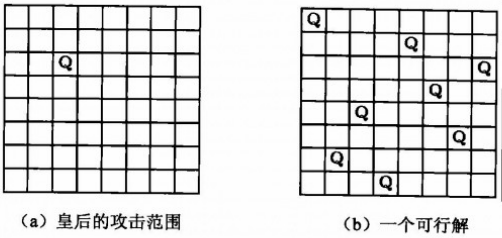
\includegraphics[width=240pt]{eight-queen.png} \\
\figcaption{八皇后问题}\label{fig:eightQueens}
\end{center}

\subsubsection{分析}
最简单的暴力枚举方法是,从64个格子中选一个子集,使得子集含有8个格子,且任意两个格子
都不在同一行、同一列或同一个对角线上。这正是子集枚举问题,然而64个格子的子集有$2^{64}$个,
太大了,这并不是一个很好的模型。

第二个思路是,从64个格子中选8个格子,这是组合生成问题。根据组合数学,有 $C_{64}^{8} \approx 4.426 \times 10^9$ 种方案,
比第一种方案优秀,但仍然不够好。

经过思考不难发现,由于每一行只能放一个皇后,那么第一行有8种选择,第二行有7中选择,…,
第8行有1中选择,总共有$8!=40320$个方案。如果用C[x]表示第x行皇后的列编号,则问题变成了一个
全排列生成问题,枚举量不会超过8!。

\subsubsection{代码}
\begin{Codex}[label=eight_queen.c]
#include <stdio.h>
#include <stdlib.h>

#define N 8 // 皇后的个数,也是棋盘的长和宽

int total = 0;  // 可行解的总数
int C[N];  // C[i]表示第i行皇后所在的列编号

/**
 * @brief 输出所有可行的棋局,按列打印.
 *
 * http://poj.grids.cn/practice/2698/ , 这题需要按列打印
 *
 * @return 无
 */
void output() {
    int i, j;
    printf("No. %d\n", total);
    for (j = 0; j < N; ++j) {
        for (i = 0; i < N; ++i) {
            if (C[i] != j) {
                printf("0 ");
            } else {
                printf("1 ");
            }
        }
        printf("\n");
    }
}

/**
 * @brief 输出所有可行的棋局,按行打印.
 * @return 无
 */
void output1() {
    int i, j;
    printf("No. %d\n", total);
    for (i = 0; i < N; ++i) {
        for (j = 0; j < N; ++j) {
            if (j != C[i]) {
                printf("0 ");
            } else {
                printf("1 ");
            }
        }
        printf("\n");
    }
}

/**
 * @brief 检查当前位置(row, column)能否放置皇后.
 *
 * @param[in] row 当前行
 * @return 能则返回1,不能则返回0
 */
int check(const int row, const int column) {
    int ok = 1;
    int i;
    for(i = 0; i < row; ++i) {
        // 两个点的坐标为(row, column), (i, C[i])
        // 检查是否在同一列,或对角线上
        if(column == C[i] || row - i == column - C[i] ||
            row - i == C[i] - column) {
            ok = 0;
            break;
        }
    }
    return ok;
}

/**
 * @brief 八皇后,深搜
 *
 * @param[in] row 搜索当前行,该在哪一列上放一个皇后
 * @return 可行解的个数
 */
int search(const int row) {
    int j;
    if (row == N) { // 终止条件,也是收敛条件,意味着找到了一个可行解
        ++total;
        output();
        return total;
    }

    for (j = 0; j < N; ++j) {  // 一列一列的试
        const int ok = check(row, j);
        if (ok) {  // 如果合法,继续递归
            C[row] = j;
            search(row + 1);
        }
    }

    return total;
}

// 表示已经放置的皇后占据了哪些列
int columns[N];
// 占据了哪些主对角线
int principal_diagonals[2 * N];
// 占据了哪些副对角线
int counter_diagonals[2 * N];

/**
 * @brief 检查当前位置(row, column)能否放置皇后.
 *
 * @param[in] row, 当前行
 * @return 能则返回1,不能则返回0
 */
int check2(const int row, const int column) {
    return columns[column] == 0 && principal_diagonals[row + column] == 0
        && counter_diagonals[row - column + N] == 0;
}

/**
 * @brief 八皇后,深搜,更优化的版本,用空间换时间
 *
 * @param[in] row 搜索当前行,该在哪一列上放一个皇后
 * @return 可行解的个数
 */
int search2(const int row) {
    int j;
    if (row == N) { // 终止条件,也是收敛条件,意味着找到了一个可行解
        ++total;
        output();
        return total;
    }

    for (j = 0; j < N; ++j) {  // 一列一列的试
        const int ok = check2(row, j);
        if (ok) {  // 如果合法,继续递归
            // 执行扩展动作
            C[row] = j;
            columns[j] = principal_diagonals[row + j] =
                    counter_diagonals[row - j + N] = 1;
            search2(row + 1);
            // 撤销动作
            C[row] = -1;  // 这句可以省略,因为C[row]会被覆盖掉
            columns[j] = principal_diagonals[row + j] =
                    counter_diagonals[row - j + N] = 0;
        }
    }

    return total;
}

int main() {
    // search(0);
    search2(0);
    return 0;
}
\end{Codex}

\subsubsection{相关的题目}
与本题相同的题目:
\begindot
\item 《算法竞赛入门经典》\footnote{刘汝佳,算法竞赛入门经典,清华大学出版社,2009} 第123页7.4.1节
\item 百练 2698 八皇后问题, \myurl{http://poj.grids.cn/practice/2698/}
\item wikioi 1295 N皇后问题, \myurl{http://www.wikioi.com/problem/1295/}
\myenddot

与本题相似的题目:
\begindot
\item POJ 1321 棋盘问题, \myurl{http://poj.org/problem?id=1321}
\myenddot


\section{还原IP地址} %%%%%%%%%%%%%%%%%%%%%%%%%%%%%%

\subsubsection{描述}
本题是 LeetCode Online Judge上的"Restore IP Addresses"。

给定一个只包含数字的字符串,还原出所有合法的IP地址。

例如:给定"25525511135",返回["255.255.11.135", "255.255.111.35"]。 (顺序无关紧要)

\subsubsection{分析}
这题很明显分为四步,有层次,因此可以尝试用回溯法解决。

\subsubsection{代码}
\begin{Codex}[label=restore_ip_adresses.cpp]
// LeetCode, Restore IP Addresses
class Solution {
public:
    vector<string> restoreIpAddresses(string s) {
        vector<string> result;
        string ip; // 存放中间结果
        dfs(s, 0, 0, ip, result);
        return result;
    }

    /**
     * @brief 解析字符串
     * @param[in] s 字符串,输入数据
     * @param[in] startIndex 从s的哪里开始
     * @param[in] step 当前步骤编号,从0开始编号,取值为0,1,2,3,4表示结束了
     * @param[out] intermediate 当前解析出来的中间结果
     * @param[out] result 存放所有可能的IP地址
     * @return 无
     */
    void dfs(string s, int start, int step, string ip,
            vector<string> &result) {
        if (s.size() - start > (4 - step) * 3)
            return;  // 非法结果,剪枝
        if (s.size() - start < (4 - step))
            return;  // 非法结果,剪枝

        if (start == s.size() && step == 4) {  // 找到一个合法解
            ip.resize(ip.size() - 1);
            result.push_back(ip);
            return;
        }

        int num = 0;
        for (int i = start; i < start + 3; i++) {
            num = num * 10 + (s[i] - '0');

            if (num <= 255) {  // 当前结点合法,则继续往下递归
                ip += s[i];
                dfs(s, i + 1, step + 1, ip + '.', result);
            }
            if (num == 0) break;  // 不允许前缀0,但允许单个0
        }
    }
};
\end{Codex}


\section{Combination Sum} %%%%%%%%%%%%%%%%%%%%%%%%%%%%%%

\subsubsection{描述}
本题是 LeetCode Online Judge上的"Combination Sum"。

给定一个数的集合(C)和一个目标数(T),找到C中所有不重复的组合,让这些被选出来的数加起来等于T。

每一个数可以被选无数次。

注意:
\begindot
\item 所有的数(包括目标)都是正整数
\item 一个组合($a_1,a_2,\cdot,a_k$)中的元素必须以非递减顺序排列
\item 一个组合不能与另一个组合重复
\myenddot

例如,给定一组数2,3,6,7,和目标7,则答案是
\begin{Code}
[7]
[2, 2, 3] 
\end{Code}

\subsubsection{分析}
这题没有固定的步骤数,但是步骤也是有限的,因此可以尝试用回溯法。

\subsubsection{代码}

\begin{Codex}[label=combination_sum.cpp]
// LeetCode, Combination Sum
class Solution {
public:
    vector<vector<int> > combinationSum(vector<int> &nums, int target) {
        sort(nums.begin(), nums.end());
        vector<vector<int> > result; // 最终结果
        vector<int> intermediate; // 中间结果
        dfs(nums, target, 0, intermediate, result);
        return result;
    }

private:
    void dfs(vector<int>& nums, int gap, int level, vector<int>& intermediate,
            vector<vector<int> > &result) {
        if (gap == 0) {  // 找到一个合法解
            result.push_back(intermediate);
            return;
        }
        for (size_t i = level; i < nums.size(); i++) { // 扩展状态
            if (gap < nums[i]) return; // 剪枝

            intermediate.push_back(nums[i]); // 执行扩展动作
            dfs(nums, gap - nums[i], i, intermediate, result);
            intermediate.pop_back();  // 撤销动作
        }
    }
};
\end{Codex}


\section{Combination Sum II} %%%%%%%%%%%%%%%%%%%%%%%%%%%%%%

\subsubsection{描述}
本题是 LeetCode Online Judge上的"Combination Sum II"。

本题与上一题唯一不同的是,每个数只能使用一次。

\subsubsection{分析}
这题没有固定的步骤数,但是步骤也是有限的,因此可以尝试用回溯法。

\subsubsection{代码}
\begin{Codex}[label=combination_sum2.cpp]
// LeetCode, Combination Sum II
class Solution {
public:
    vector<vector<int> > combinationSum2(vector<int> &nums, int target) {
        sort(nums.begin(), nums.end()); // 跟第 50 行配合,
                                             // 确保每个元素最多只用一次
        vector<vector<int> > result;
        vector<int> intermediate;
        dfs(nums, target, 0, intermediate, result);
        return result;
    }
private:
    // 使用nums[index, nums.size())之间的元素,能找到的所有可行解
    static void dfs(vector<int> &nums, int gap, int index,
            vector<int> &intermediate, vector<vector<int> > &result) {
        if (gap == 0) {  //  找到一个合法解
            result.push_back(intermediate);
            return;
        }

        int previous = -1;
        for (size_t i = index; i < nums.size(); i++) {
            // 如果上一轮循环没有选nums[i],则本次循环就不能再选nums[i],
            // 确保nums[i]最多只用一次
            if (previous == nums[i]) continue;

            if (gap < nums[i]) return;  // 剪枝

            previous = nums[i];

            intermediate.push_back(nums[i]);
            dfs(nums, gap - nums[i], i + 1, intermediate, result);
            intermediate.pop_back();  // 恢复环境
        }
    }
};
\end{Codex}


\section{小结} %%%%%%%%%%%%%%%%%%%%%%%%%%%%%%
\label{sec:dfs-template}


\subsection{适用场景}

注意,这里的总结是一种经验,一种概率,不是绝对的结论!

\textbf{输入数据}:如果是递归数据结构,如单链表,二叉树,集合,则百分之百可以用深搜;如果是非递归数据结构,如一维数组,二维数组,字符串,图,则概率小一些。

\textbf{状态转换图}:树或者图。

\textbf{求解目标}:必须要走到最深(例如对于树,必须要走到叶子节点)才能得到一个解,这种情况适合用深搜。


\subsection{思考的步骤}
\begin{enumerate}
\item 是求路径条数,还是路径本身(或动作序列)?深搜最常见的三个问题,求可行解的总数,求一个可行解,求所有可行解。
    \begin{enumerate}
    \item 如果是求路径本身,则要用一个数组\fn{path[]}存储路径。跟宽搜不同,宽搜虽然最终求的也是一条路径,但是需要存储扩展过程中的所有路径,在没找到答案之前所有路径都不能放弃;而深搜,在搜索过程中始终只有一条路径,因此用一个数组就足够了。
    \item 如果是路径条数,则不需要存储路径。
    \end{enumerate}

\item 只要求一个解,还是要求所有解?如果只要求一个解,那找到一个就可以返回;如果要求所有解,找到了一个后,还要继续扩展,直到遍历完。广搜一般只要求一个解,因而不需要考虑这个问题(广搜当然也可以求所有解,这时需要扩展到所有叶子节点,相当于在内存中存储整个状态转换图,非常占内存,因此广搜不适合解这类问题)。

\item 如何表示状态?即一个状态需要存储哪些些必要的数据,才能够完整提供如何扩展到下一步状态的所有信息。跟广搜不同,深搜的惯用写法,不是把数据记录在状态\fn{struct}里,而是添加函数参数(有时为了节省递归堆栈,用全局变量),\fn{struct}里的字段与函数参数一一对应。

\item 如何扩展状态?这一步跟上一步相关。状态里记录的数据不同,扩展方法就不同。对于固定不变的数据结构(一般题目直接给出,作为输入数据),如二叉树,图等,扩展方法很简单,直接往下一层走,对于隐式图,要先在第1步里想清楚状态所带的数据,想清楚了这点,那如何扩展就很简单了。

\item 关于判重
    \begin{enumerate}
    \item 如果状态转换图是一棵树,则不需要判重,因为在遍历过程中不可能重复。
    \item 如果状态转换图是一个图,则需要判重,方法跟广搜相同,见第 \S \ref{sec:bfs-template} 节。这里跟第8步中的加缓存是相同的,如果有重叠子问题,则需要判重,此时加缓存自然也是有效果的。
    \end{enumerate}

\item 终止条件是什么?终止条件是指到了不能扩展的末端节点。对于树,是叶子节点,对于图或隐式图,是出度为0的节点。

\item {收敛条件是什么?收敛条件是指找到了一个合法解的时刻。如果是正向深搜(父状态处理完了才进行递归,即父状态不依赖子状态,递归语句一定是在最后,尾递归),则是指是否达到目标状态;如果是逆向深搜(处理父状态时需要先知道子状态的结果,此时递归语句不在最后),则是指是否到达初始状态。

由于很多时候终止条件和收敛条件是是合二为一的,因此很多人不区分这两种条件。仔细区分这两种条件,还是很有必要的。

为了判断是否到了收敛条件,要在函数接口里用一个参数记录当前的位置(或距离目标还有多远)。如果是求一个解,直接返回这个解;如果是求所有解,要在这里收集解,即把第一步中表示路径的数组\fn{path[]}复制到解集合里。}

\item 如何加速?
    \begin{enumerate}
    \item 剪枝。深搜一定要好好考虑怎么剪枝,成本小收益大,加几行代码,就能大大加速。这里没有通用方法,只能具体问题具体分析,要充分观察,充分利用各种信息来剪枝,在中间节点提前返回。
    \item 缓存。如果子问题的解会被重复利用,可以考虑使用缓存。
        \begin{enumerate}
            \item 前提条件:子问题的解会被重复利用,即子问题之间的依赖关系是有向无环图(DAG)。如果依赖关系是树状的(例如树,单链表),没必要加缓存,因为子问题只会一层层往下,用一次就再也不会用到,加了缓存也没什么加速效果。
            \item 具体实现:可以用数组或HashMap。维度简单的,用数组;维度复杂的,用HashMap,C++有\fn{map},C++ 11以后有\fn{unordered_map},比\fn{map}快。
        \end{enumerate}
    
    \end{enumerate}
\end{enumerate}

拿到一个题目,当感觉它适合用深搜解决时,在心里面把上面8个问题默默回答一遍,代码基本上就能写出来了。对于树,不需要回答第5和第8个问题。如果读者对上面的经验总结看不懂或感觉“不实用”,很正常,因为这些经验总结是笔者做了很多深搜题后总结出来的,从思维的发展过程看,“经验总结”要晚于感性认识,所以这时候建议读者先做做后面的题目,积累一定的感性认识后,在回过头来看这一节的总结,相信会和笔者有共鸣。


\subsection{代码模板}

\begin{Codex}[label=dfs_template.c]
/**
 * dfs模板.
 * @param[in] input 输入数据指针
 * @param[inout] cur or gap 标记当前位置或距离目标的距离
 * @param[out] path 当前路径,也是中间结果
 * @param[out] result 存放最终结果
 * @return 路径长度,如果是求路径本身,则不需要返回长度
 */
void dfs(type *input, type *path, int cur or gap, type *result) {
    if (数据非法) return 0;   // 终止条件
    if (cur == input.size( or gap == 0)) { // 收敛条件
        将path放入result
    }

    if (可以剪枝) return;

    for(...) { // 执行所有可能的扩展动作
        执行动作,修改path
        dfs(input, step + 1 or gap--, result);
        恢复path
    }
}
\end{Codex}


\subsection{深搜与回溯法的区别}
深搜(Depth-first search, DFS)的定义见\myurl{http://en.wikipedia.org/wiki/Depth_first_search},回溯法(backtracking)的定义见\myurl{http://en.wikipedia.org/wiki/Backtracking}

\textbf{回溯法 = 深搜 + 剪枝}。一般大家用深搜时,或多或少会剪枝,因此深搜与回溯法没有什么不同,可以在它们之间画上一个等号。本书同时使用深搜和回溯法两个术语,但读者可以认为二者等价。

深搜一般用递归(recursion)来实现,这样比较简洁。

深搜能够在候选答案生成到一半时,就进行判断,抛弃不满足要求的答案,所以深搜比暴力搜索法要快。


\subsection{深搜与递归的区别}
深搜经常用递归(recursion)来实现,二者常常同时出现,导致很多人误以为他俩是一个东西。

深搜,是逻辑意义上的算法,递归,是一种物理意义上的实现,它和迭代(iteration)是对应的。深搜,可以用递归来实现,也可以用栈来实现;而递归,一般总是用来实现深搜。可以说,\textbf{递归一定是深搜,深搜不一定用递归}。

递归有两种加速策略,一种是\textbf{剪枝(prunning)},对中间结果进行判断,提前返回;一种是\textbf{加缓存}(就变成了memoization,备忘录法),缓存中间结果,防止重复计算,用空间换时间。

其实,递归+缓存,就是一种 memorization 。所谓\textbf{memorization}(翻译为备忘录法,见第 \S \ref{sec:dp-vs-memorization}节),就是"top-down with cache"(自顶向下+缓存),它是Donald Michie 在1968年创造的术语,表示一种优化技术,在top-down 形式的程序中,使用缓存来避免重复计算,从而达到加速的目的。

\textbf{memorization 不一定用递归},就像深搜不一定用递归一样,可以在迭代(iterative)中使用 memorization 。\textbf{递归也不一定用 memorization},可以用memorization来加速,但不是必须的。只有当递归使用了缓存,它才是 memorization 。

既然递归一定是深搜,为什么很多书籍都同时使用这两个术语呢?在递归味道更浓的地方,一般用递归这个术语,在深搜更浓的场景下,用深搜这个术语,读者心里要弄清楚他俩大部分时候是一回事。在单链表、二叉树等递归数据结构上,递归的味道更浓,这时用递归这个术语;在图、隐士图等数据结构上,递归的比重不大,深搜的意图更浓,这时用深搜这个术语。
